% -*- mode: noweb; noweb-default-code-mode: R-mode; -*-
\documentclass[a4paper]{article}

\title{A Test File}
\author{Friedrich Leisch}


\usepackage{a4wide}

\usepackage{/usr/lib/R/share/texmf/Sweave}
\begin{document}

\maketitle

A simple example that will run in any S engine: The integers from 1 to
10 are
\begin{Schunk}
\begin{Soutput}
 [1]  1  2  3  4  5  6  7  8  9 10
\end{Soutput}
\end{Schunk}

We can also emulate a simple calculator:
\begin{Schunk}
\begin{Sinput}
> 1 + 1
\end{Sinput}
\begin{Soutput}
[1] 2
\end{Soutput}
\begin{Sinput}
> 1 + pi
\end{Sinput}
\begin{Soutput}
[1] 4.141593
\end{Soutput}
\begin{Sinput}
> sin(pi/2)
\end{Sinput}
\begin{Soutput}
[1] 1
\end{Soutput}
\end{Schunk}

Now we look at Gaussian data:

\begin{Schunk}
\begin{Soutput}
 [1] -0.39658933  0.97984991 -0.48227328  0.02366086 -1.20264425  0.90590844
 [7]  1.09473606  0.64457102 -0.87791805 -0.67595809  0.45706530  0.14519694
[13]  1.01439743  1.06458523  0.27494175 -0.55222331 -0.05722188 -0.92387674
[19] -1.29543431  1.79094102
\end{Soutput}
\begin{Soutput}
	One Sample t-test

data:  x 
t = 0.4896, df = 19, p-value = 0.63
alternative hypothesis: true mean is not equal to 0 
95 percent confidence interval:
 -0.3163053  0.5094767 
sample estimates:
 mean of x 
0.09658574 
\end{Soutput}
\end{Schunk}
Note that we can easily integrate some numbers into standard text: The
third element of vector \texttt{x} is -0.482273282274676, the
$p$-value of the test is 0.63001. % $

Now we look at a summary of the famous iris data set, and we want to
see the commands in the code chunks.  Note that the summary needs to
be \texttt{print()}ed explicitly, because eval would discard it otherwise. I
consider this a feature, because it allows for much finer control on
what gets into the final report.



% the following code is R-specific, as data(iris) will not run in Splus.
% Hence, we mark it as R code.
\begin{Schunk}
\begin{Sinput}
> data(iris)
> print(summary(iris))
\end{Sinput}
\begin{Soutput}
  Sepal.Length    Sepal.Width     Petal.Length    Petal.Width   
 Min.   :4.300   Min.   :2.000   Min.   :1.000   Min.   :0.100  
 1st Qu.:5.100   1st Qu.:2.800   1st Qu.:1.600   1st Qu.:0.300  
 Median :5.800   Median :3.000   Median :4.350   Median :1.300  
 Mean   :5.843   Mean   :3.057   Mean   :3.758   Mean   :1.199  
 3rd Qu.:6.400   3rd Qu.:3.300   3rd Qu.:5.100   3rd Qu.:1.800  
 Max.   :7.900   Max.   :4.400   Max.   :6.900   Max.   :2.500  
       Species  
 setosa    :50  
 versicolor:50  
 virginica :50  
\end{Soutput}
\end{Schunk}


\begin{figure}[htbp]
  \begin{center}
\begin{Schunk}
\begin{Sinput}
> library(graphics)
> pairs(iris)
\end{Sinput}
\end{Schunk}
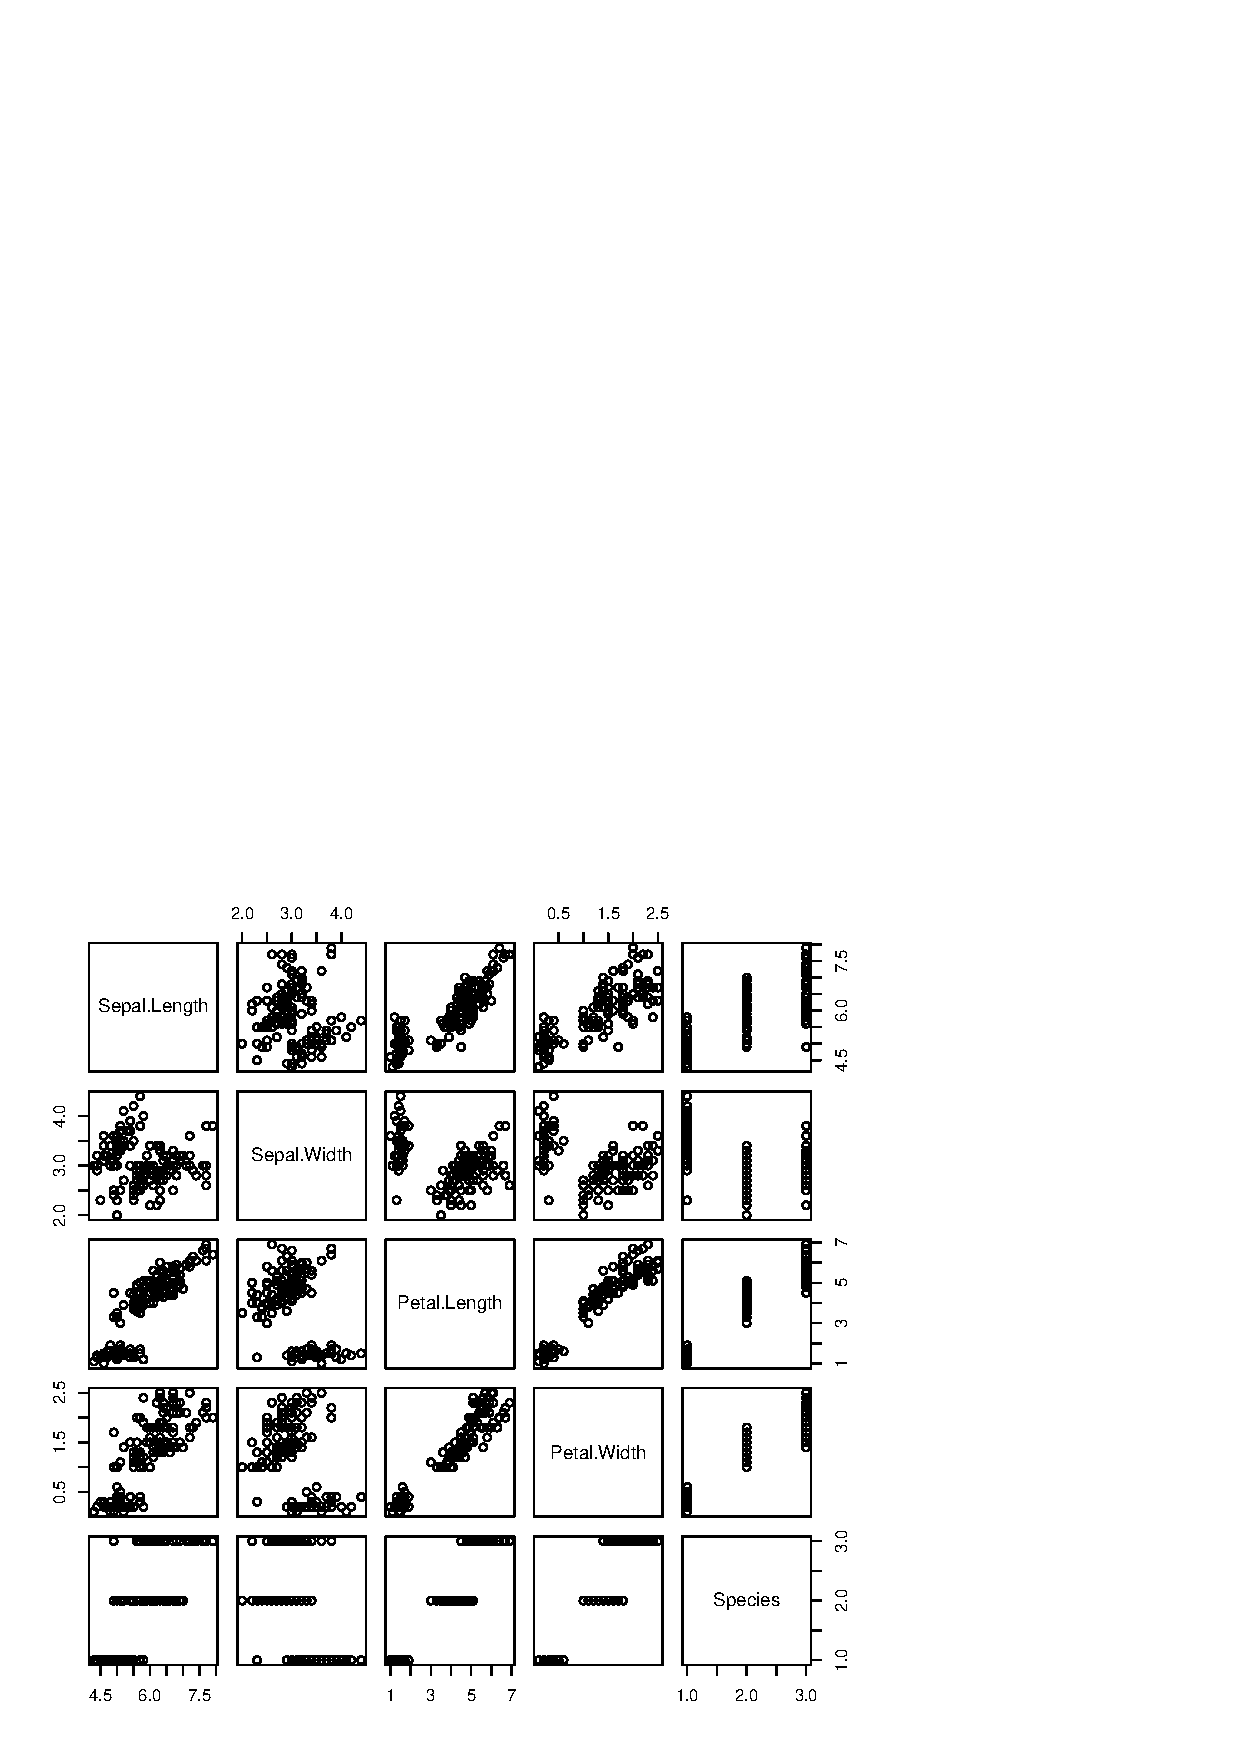
\includegraphics{Sweave-test-1-006}
    \caption{Pairs plot of the iris data.}
  \end{center}
\end{figure}

\begin{figure}[htbp]
  \begin{center}
\begin{Schunk}
\begin{Sinput}
> boxplot(Sepal.Length ~ Species, data = iris)
\end{Sinput}
\end{Schunk}
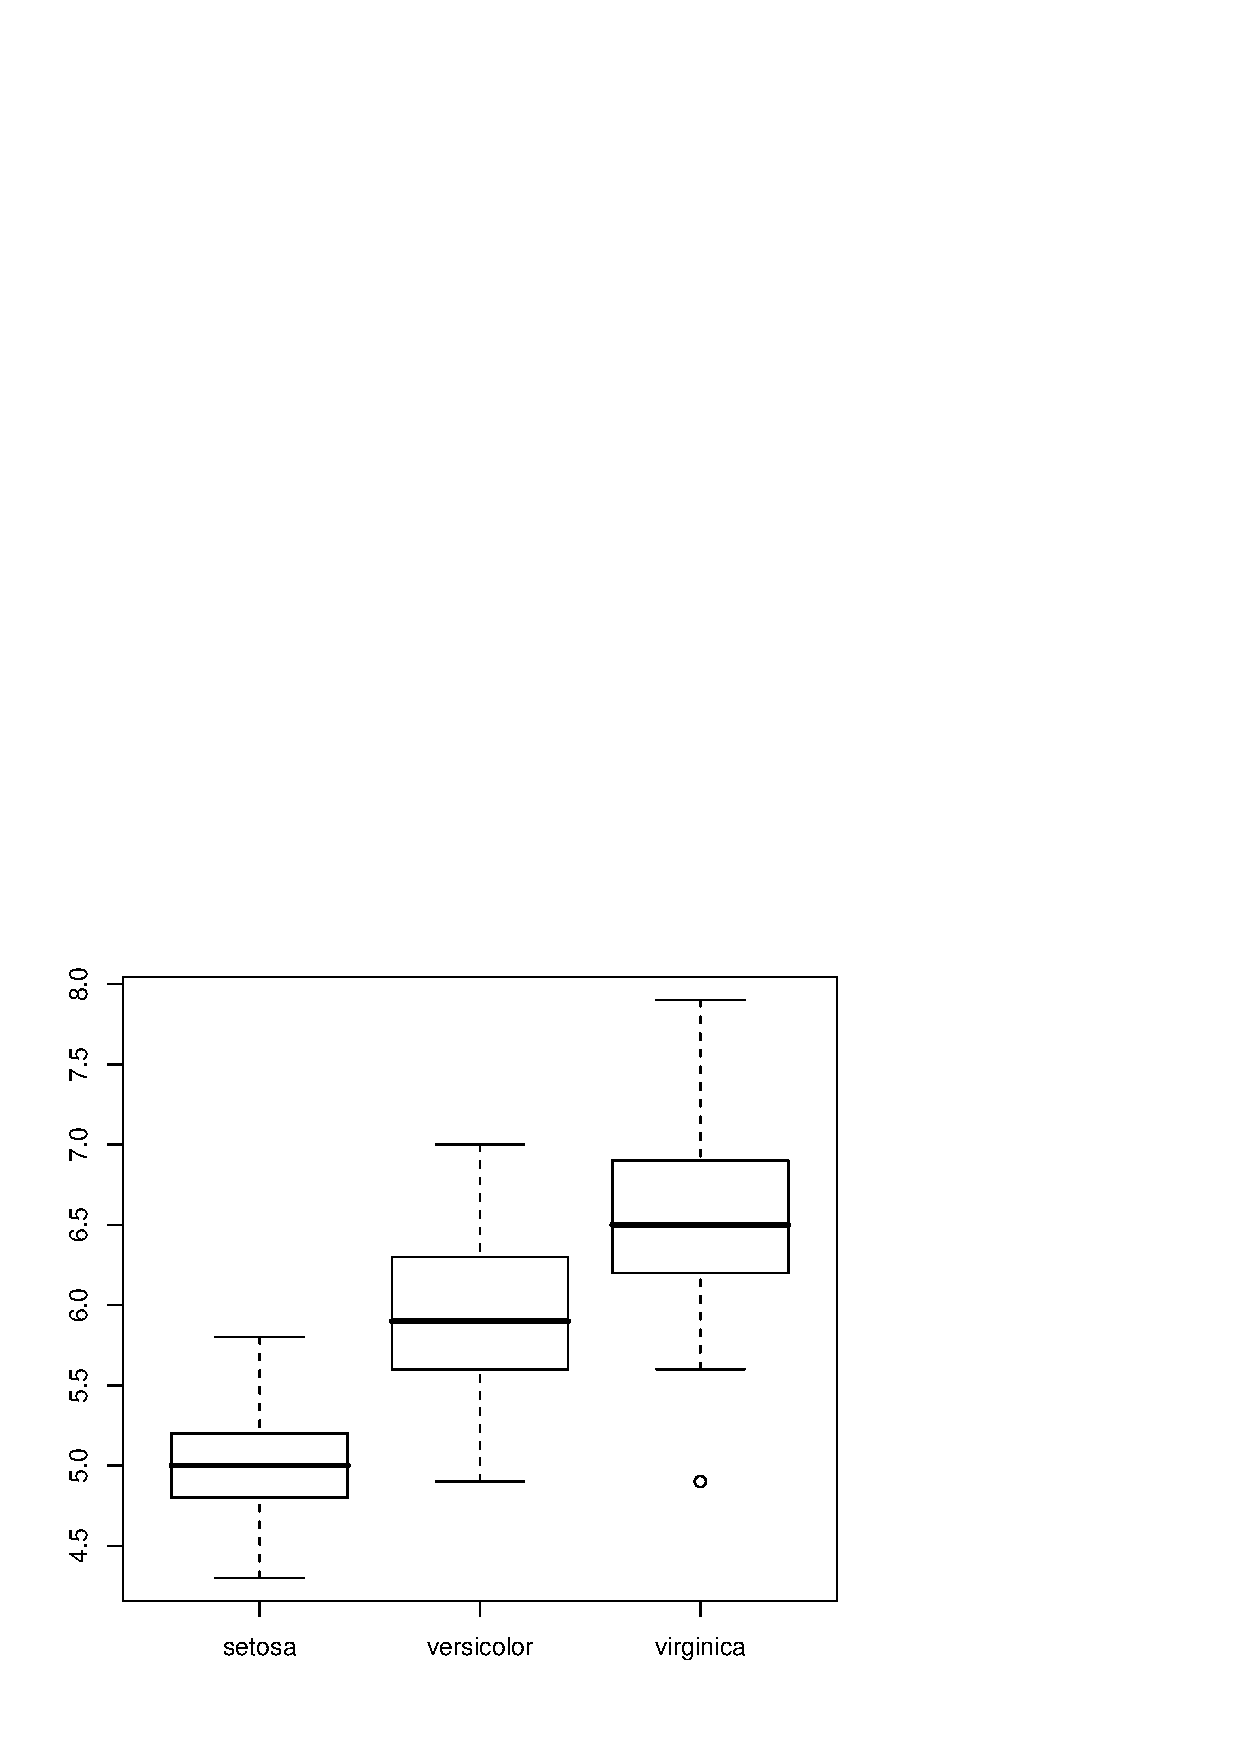
\includegraphics{Sweave-test-1-007}
    \caption{Boxplot of sepal length grouped by species.}
  \end{center}
\end{figure}


% R is not S-PLUS, hence this chunk will be ignored:

\end{document}


